

\tikzset{every picture/.style={line width=0.75pt}} %set default line width to 0.75pt        

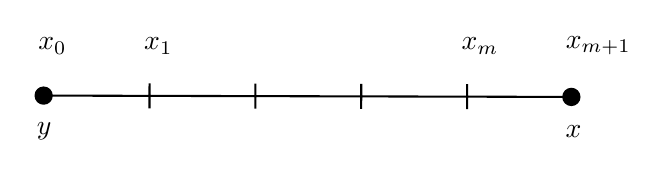
\begin{tikzpicture}[x=0.75pt,y=0.75pt,yscale=-1.5,xscale=1.5]
%uncomment if require: \path (0,68.99998474121094); %set diagram left start at 0, and has height of 68.99998474121094

%Straight Lines [id:da38713666625893595] 
\draw    (233.5,39) -- (403,39.43) (267.51,35.09) -- (267.49,43.09)(301.51,35.17) -- (301.49,43.17)(335.51,35.26) -- (335.49,43.26)(369.51,35.34) -- (369.49,43.34) ;


%Shape: Circle [id:dp053632030794002805] 
\draw  [fill={rgb, 255:red, 0; green, 0; blue, 0 }  ,fill opacity=1 ] (230.9,39) .. controls (230.9,37.56) and (232.06,36.4) .. (233.5,36.4) .. controls (234.94,36.4) and (236.1,37.56) .. (236.1,39) .. controls (236.1,40.44) and (234.94,41.6) .. (233.5,41.6) .. controls (232.06,41.6) and (230.9,40.44) .. (230.9,39) -- cycle ;
%Shape: Circle [id:dp6730801146643859] 
\draw  [fill={rgb, 255:red, 0; green, 0; blue, 0 }  ,fill opacity=1 ] (400.4,39.43) .. controls (400.4,37.99) and (401.56,36.82) .. (403,36.82) .. controls (404.44,36.82) and (405.6,37.99) .. (405.6,39.43) .. controls (405.6,40.87) and (404.44,42.03) .. (403,42.03) .. controls (401.56,42.03) and (400.4,40.87) .. (400.4,39.43) -- cycle ;

% Text Node
\draw (233.67,50.43) node   {$y$};
% Text Node
\draw (236.33,23.1) node   {$x_{0}$};
% Text Node
\draw (270.33,23.1) node   {$x_{1}$};
% Text Node
\draw (403.67,50.43) node   {$x$};
% Text Node
\draw (373.67,23.1) node   {$x_{m}$};
% Text Node
\draw (411.67,23.1) node   {$x_{m+1}$};


\end{tikzpicture}
